\section{可视化效果}

\subsection{交互参数与页面组织}

本项目的网页界面基于Streamlit实现。
左侧参数栏用于设置实验条件，包括量子比特数、目标态、最大Grover迭代次数，
以及是否显示statevector表格、Qiskit电路图和理想/带噪声实验对照。
主页面按照观察Grover算法的自然顺序组织：
先观察单步状态变化，再观察完整迭代后的目标态概率曲线，
随后查看量子电路结构，最后对比理想模拟和带噪声模拟结果。

图~\ref{fig:web-sidebar}展示了页面左侧的参数控制区域。
基础参数区用于选择量子比特数、目标态和最大Grover迭代次数，
这三个参数决定搜索空间大小、Oracle标记的目标态以及需要展示的演化步数。
% 这里的“最大Grover迭代次数”表示页面生成曲线和步进历史时保留到第几轮完整Grover迭代，
% 并不意味着所有图都只展示最终一步。
显示选项区用于控制是否展示statevector表格、Qiskit电路结构以及理想/带噪声实验对照。
高级噪声参数区用于设置带噪声Aer模拟中的shots数量、单比特门错误率、双比特门错误率和读出错误率。
通过这些参数，用户可以在同一界面中观察理想Grover演化和带噪声测量结果之间的差异。

\begin{figure}[H]
  \centering
  \IfFileExists{images/web_crops/sidebar_combined.png}{
    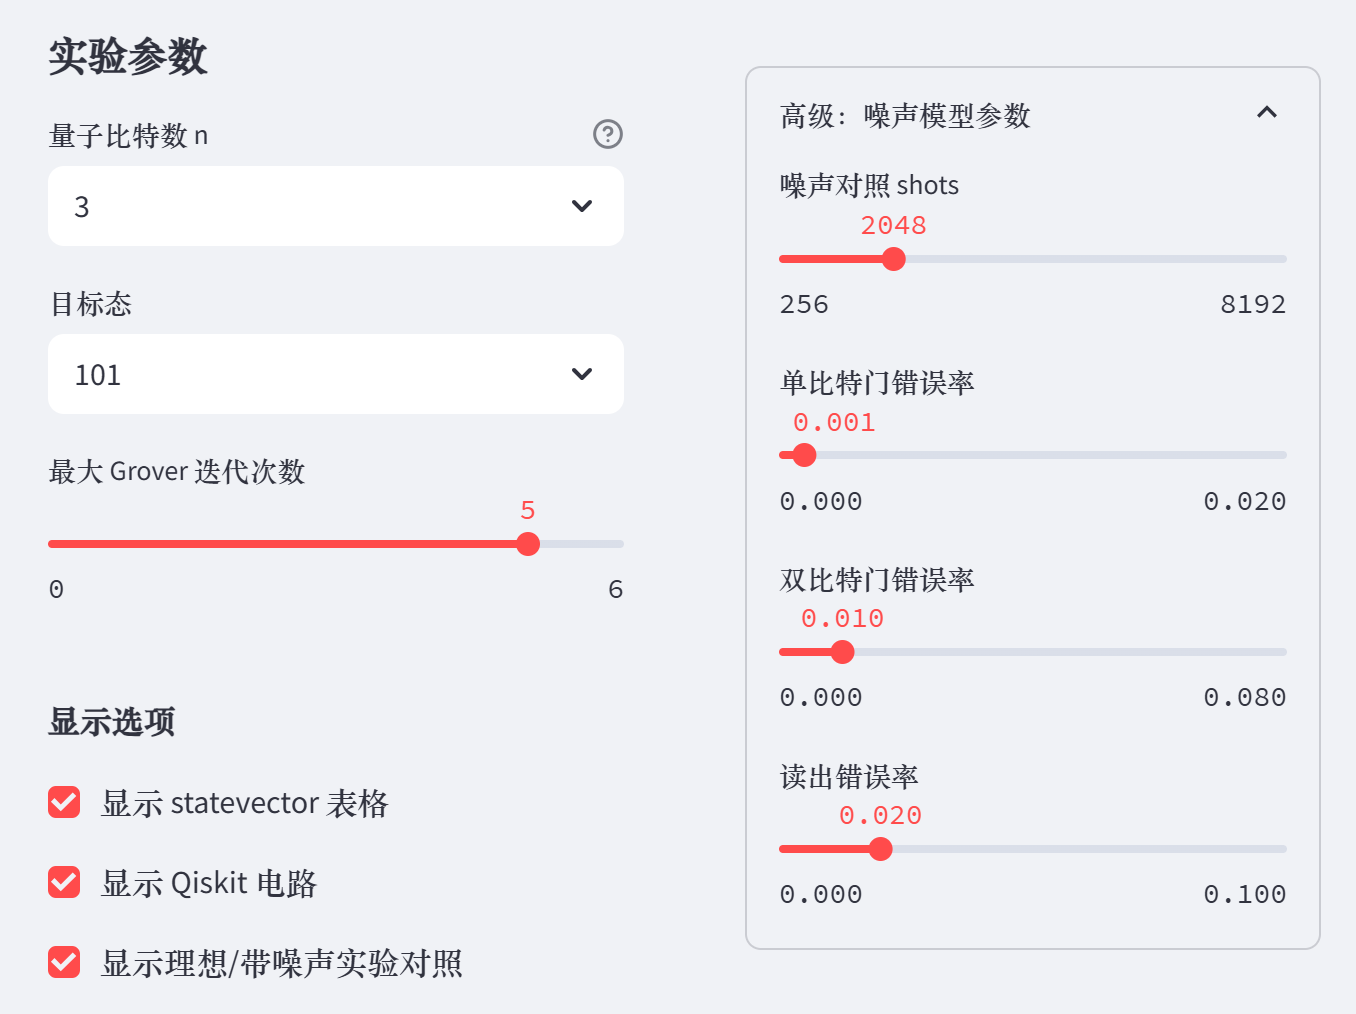
\includegraphics[width=0.95\textwidth]{images/web_crops/sidebar_combined.png}
  }{
    \fbox{\parbox[c][5cm][c]{0.9\textwidth}{\centering 待插入侧边栏参数截图}}
  }
  \caption{Streamlit侧边栏中的实验参数设置}
  \label{fig:web-sidebar}
\end{figure}

\subsection{步进式概率幅与概率展示}

图~\ref{fig:web-step-view}展示了当前步骤的可视化界面。
页面上方给出目标态、总演化步骤数、最高目标态概率和经验最佳迭代次数等摘要信息；
中间区域通过“上一步”“下一步”和滑块选择不同演化步骤；
下方两张柱状图分别显示当前statevector中各计算基态的实数概率幅和测量概率。
目标态使用橙色突出显示。
% Oracle步骤后，目标态概率幅的符号发生翻转，但测量概率保持不变；
% Diffusion步骤后，目标态概率幅被推高，对应的测量概率明显上升。

\begin{figure}[H]
  \centering
  \IfFileExists{images/web_crops/web_step_view.png}{
    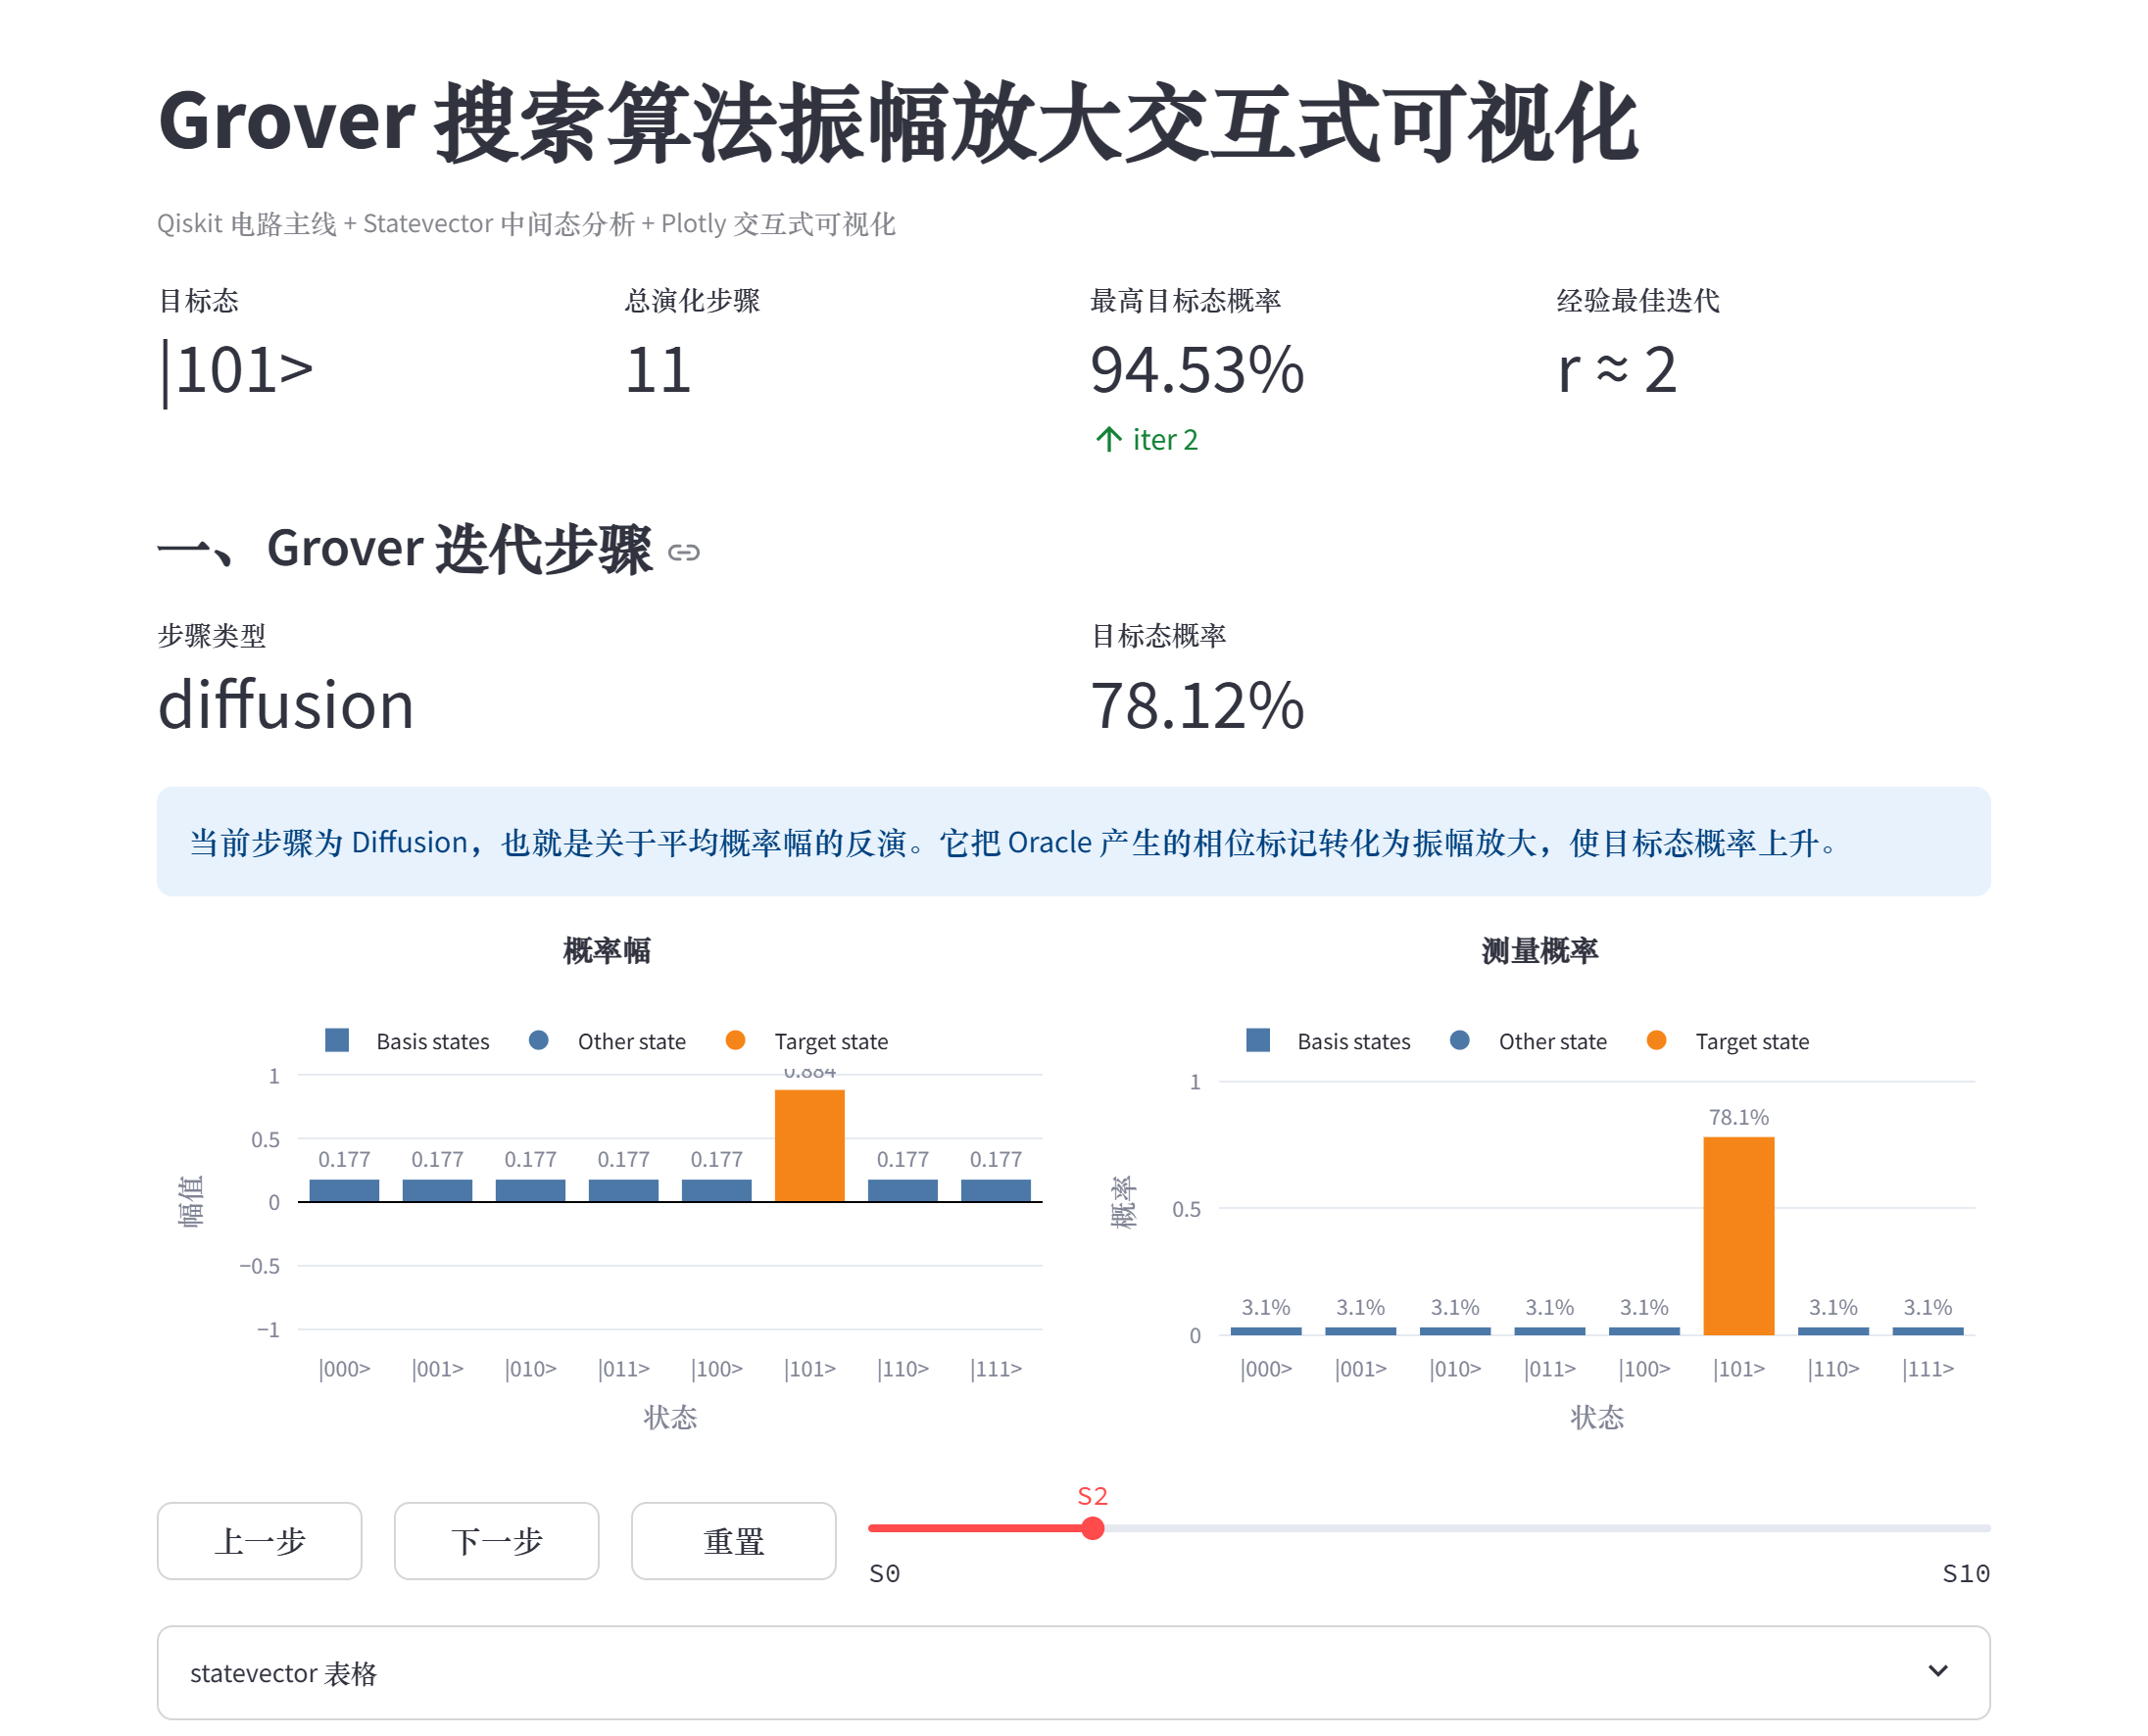
\includegraphics[width=0.95\textwidth]{images/web_crops/web_step_view.png}
  }{
    \fbox{\parbox[c][5cm][c]{0.9\textwidth}{\centering 待插入当前步骤页面截图}}
  }
  \caption{Grover算法当前步骤的概率幅与测量概率可视化界面}
  \label{fig:web-step-view}
\end{figure}

\subsection{目标态概率曲线}

除了单步柱状图外，页面还绘制了目标态概率随完整Grover迭代次数变化的曲线，
如图~\ref{fig:web-target-curve}所示。
该图以完整迭代次数为横轴，以目标态测量概率为纵轴，
用于观察目标态概率在多次Grover迭代中的整体变化趋势。
若侧边栏中最大迭代次数设为5，则曲线会展示\(r=0\)到\(r=5\)的目标态概率；
其中\(r=0\)表示只完成Hadamard初始化，尚未执行Oracle和Diffusion。

对于\(n=3\)、单目标态搜索的示例，第一次完整Grover迭代后目标态概率已经明显升高，
第二次迭代后进一步接近峰值。
该曲线也说明Grover算法并不是迭代次数越多越好，当迭代超过合适次数后，目标态概率会出现回落。
% 因此，页面同时给出经验最佳迭代次数，帮助解释Grover算法中迭代次数选择的重要性。

\begin{figure}[H]
  \centering
  \IfFileExists{images/web_crops/web_target_curve.png}{
    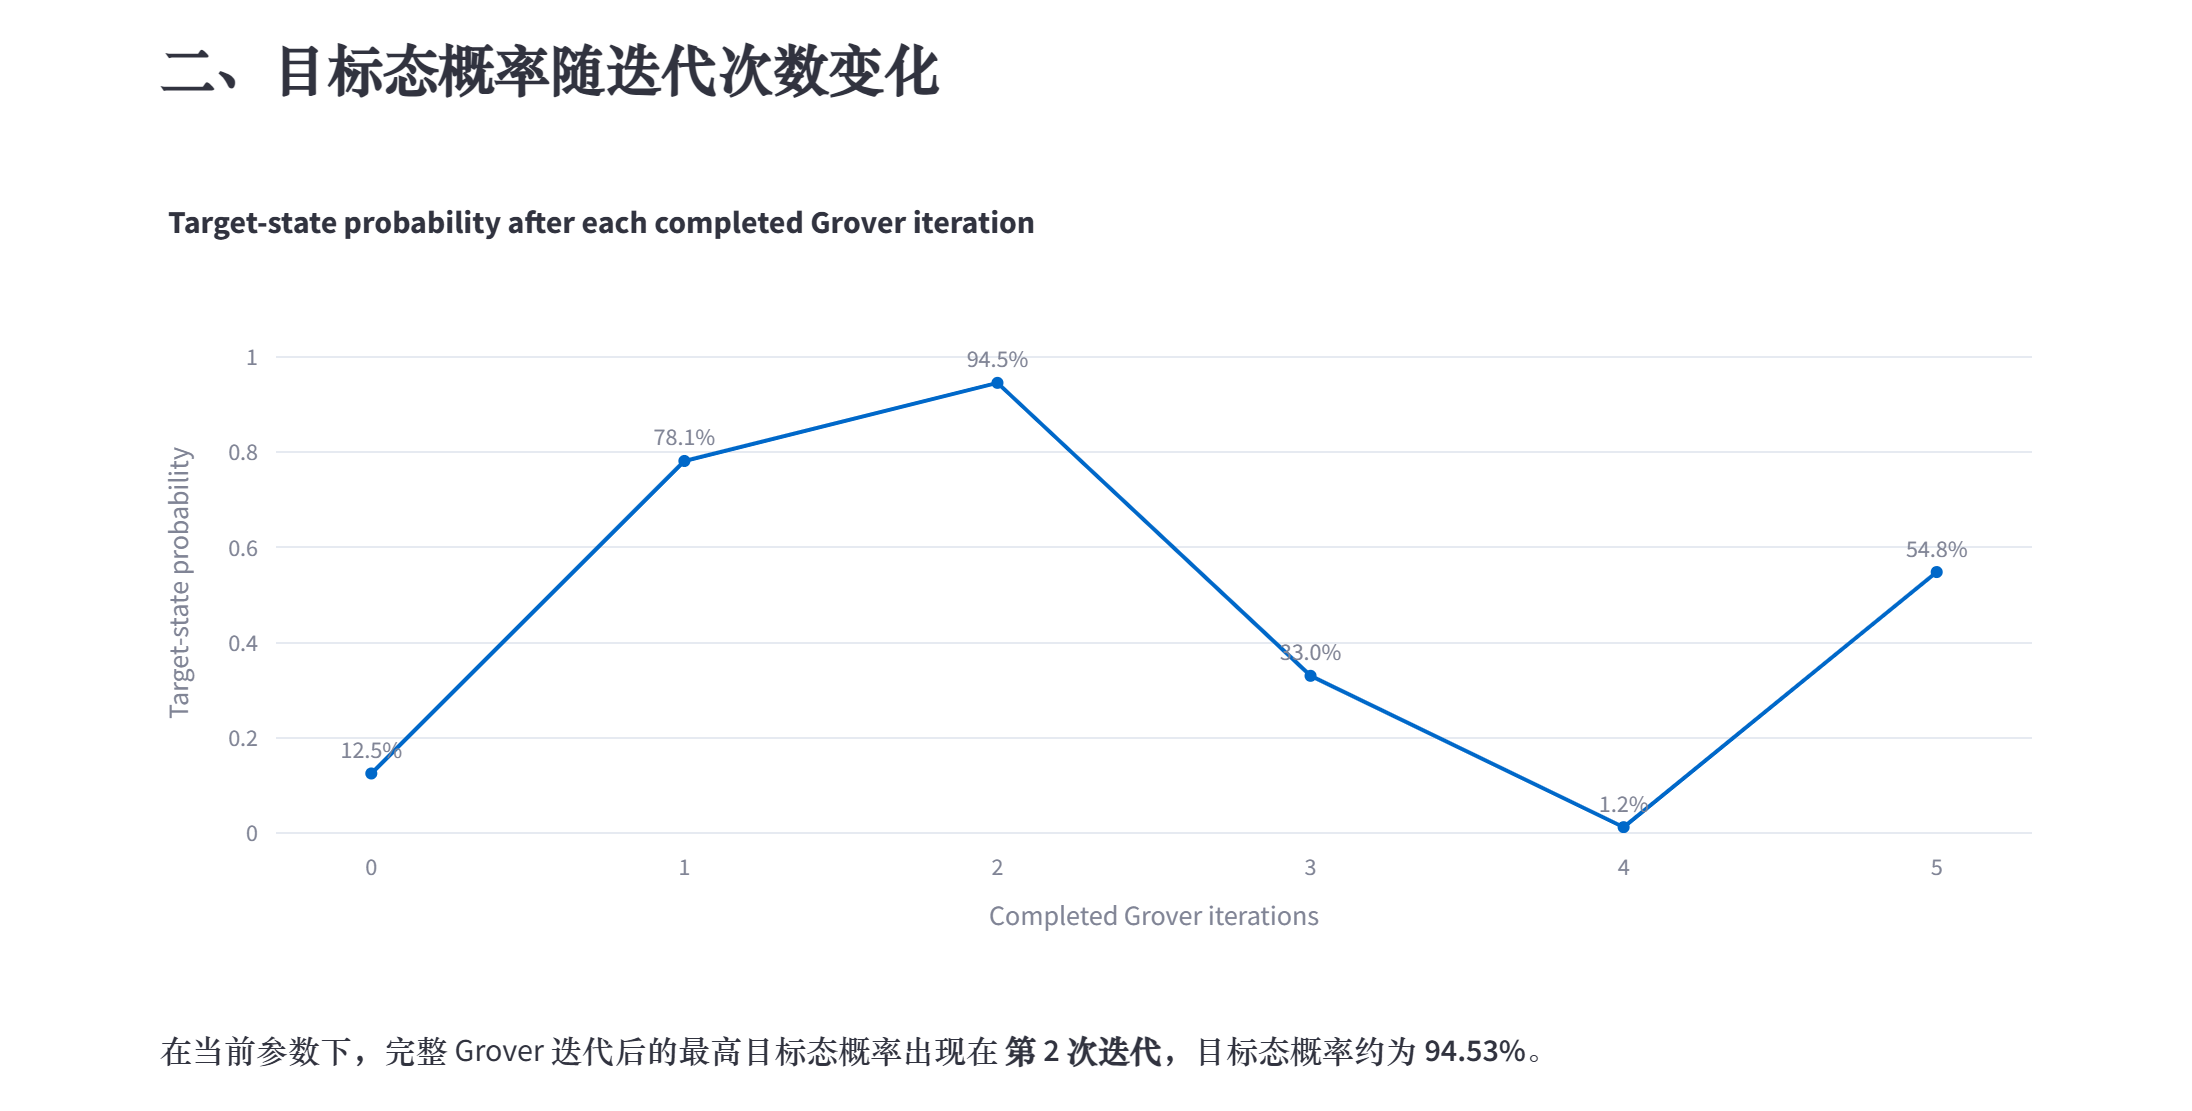
\includegraphics[width=0.88\textwidth]{images/web_crops/web_target_curve.png}
  }{
    \fbox{\parbox[c][5cm][c]{0.9\textwidth}{\centering 待插入目标态概率曲线截图}}
  }
  \caption{目标态概率随完整Grover迭代次数变化的曲线}
  \label{fig:web-target-curve}
\end{figure}

\subsection{Qiskit量子电路结构展示}

图~\ref{fig:web-circuit-view}展示了Qiskit量子电路的交互式操作视图。
该视图将Hadamard初始化、Oracle、Diffusion和测量操作按照电路时间顺序展开，
并保留量子比特线路之间的连接关系。
这一视图能够说明概率幅变化所来自的具体的量子门操作。

在实现上，页面同时提供交互式操作视图、操作表和Qiskit标准电路图三个入口。
交互式操作视图适合观察门操作的顺序和类型，操作表适合检查每一步电路指令，
标准电路图则用于和Qiskit原生绘图结果对照。

\begin{figure}[H]
  \centering
  \IfFileExists{images/web_crops/web_circuit_view.png}{
    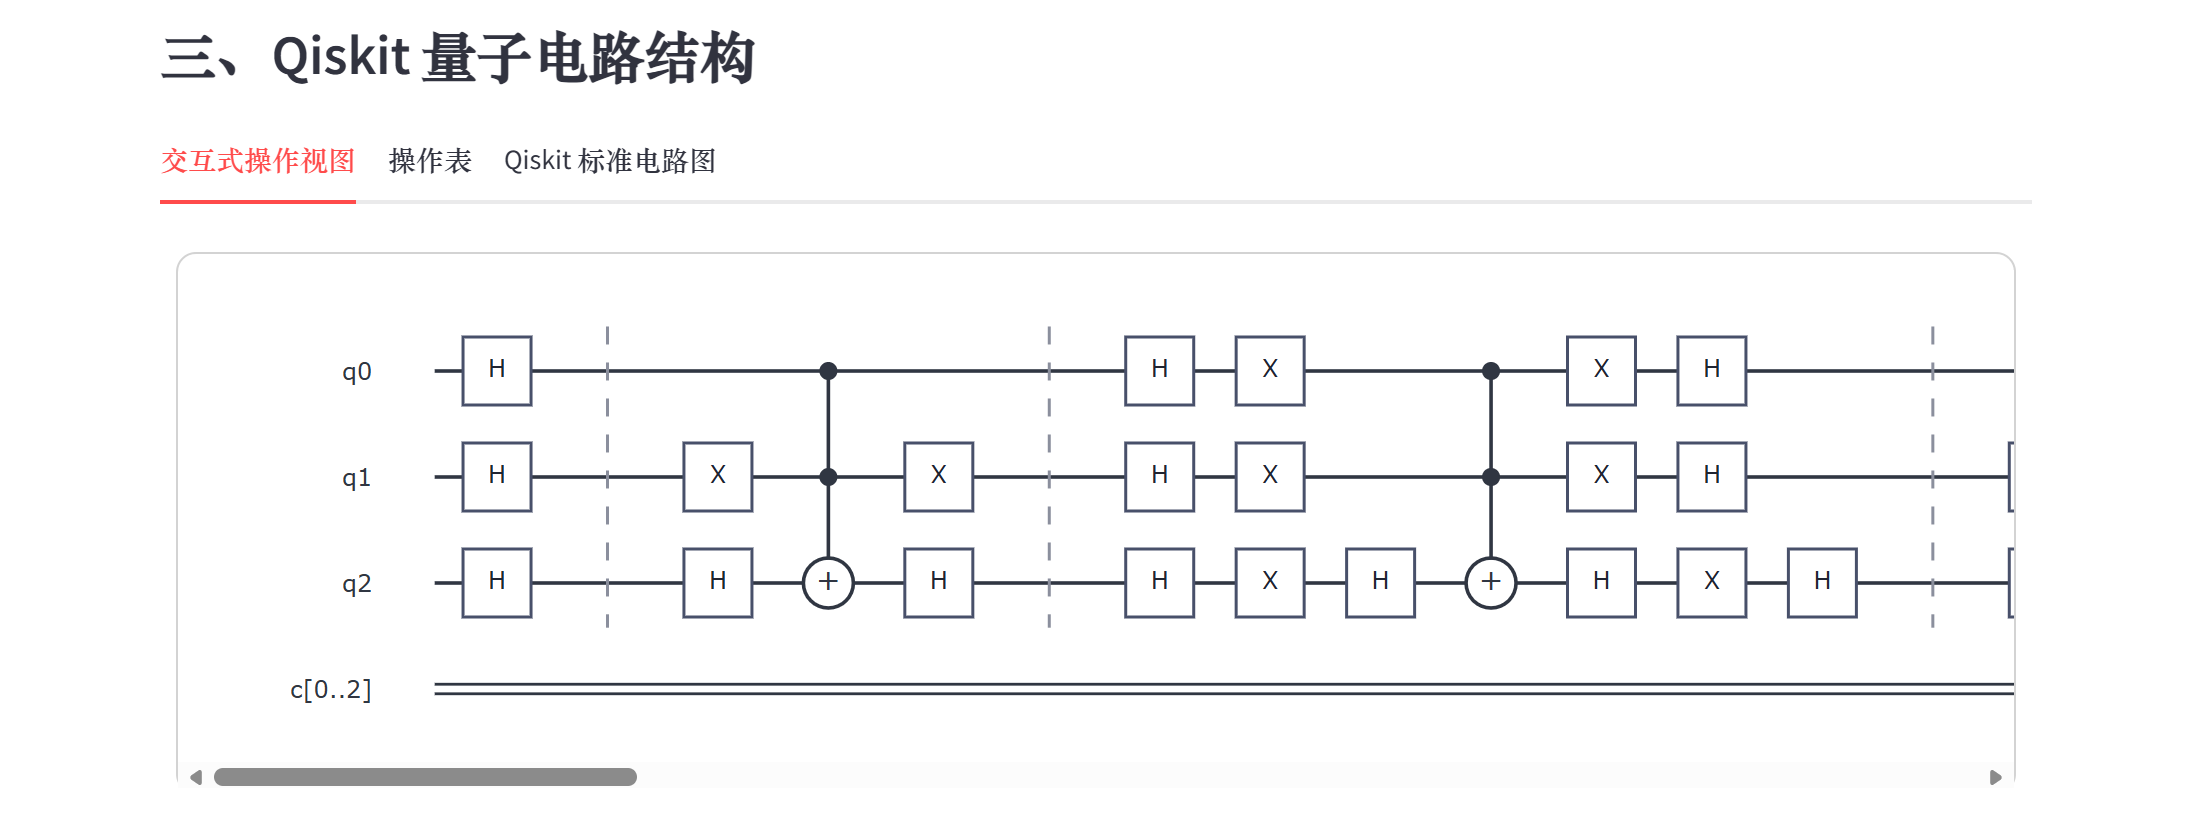
\includegraphics[width=0.95\textwidth]{images/web_crops/web_circuit_view.png}
  }{
    \fbox{\parbox[c][5cm][c]{0.9\textwidth}{\centering 待插入Qiskit电路结构页面截图}}
  }
  \caption{Qiskit量子电路的交互式操作视图}
  \label{fig:web-circuit-view}
\end{figure}

\subsection{理想与带噪声实验对照}

为展示量子电路在带噪声条件下的表现，
页面加入了理想statevector结果与带噪声Aer模拟结果的对照模块，
如图~\ref{fig:web-noise-view}所示。
该模块给出理想目标态概率、带噪声测量频率、目标态损耗、电路深度和CX门数量等摘要指标，
并提供三维分布对照和目标态损耗曲线两个视图。

三维分布对照视图可以在“理想概率分布”“带噪声测量频率”和“理想--带噪声差值”之间切换。
三维分布图说明，当电路深度和多比特门数量增加时，带噪声测量结果会偏离理想概率分布。
目标态损耗曲线则从整体趋势上展示理想概率与带噪声频率之间的差异。

\begin{figure}[H]
  \centering
  \IfFileExists{images/web_crops/web_noise_view.png}{
    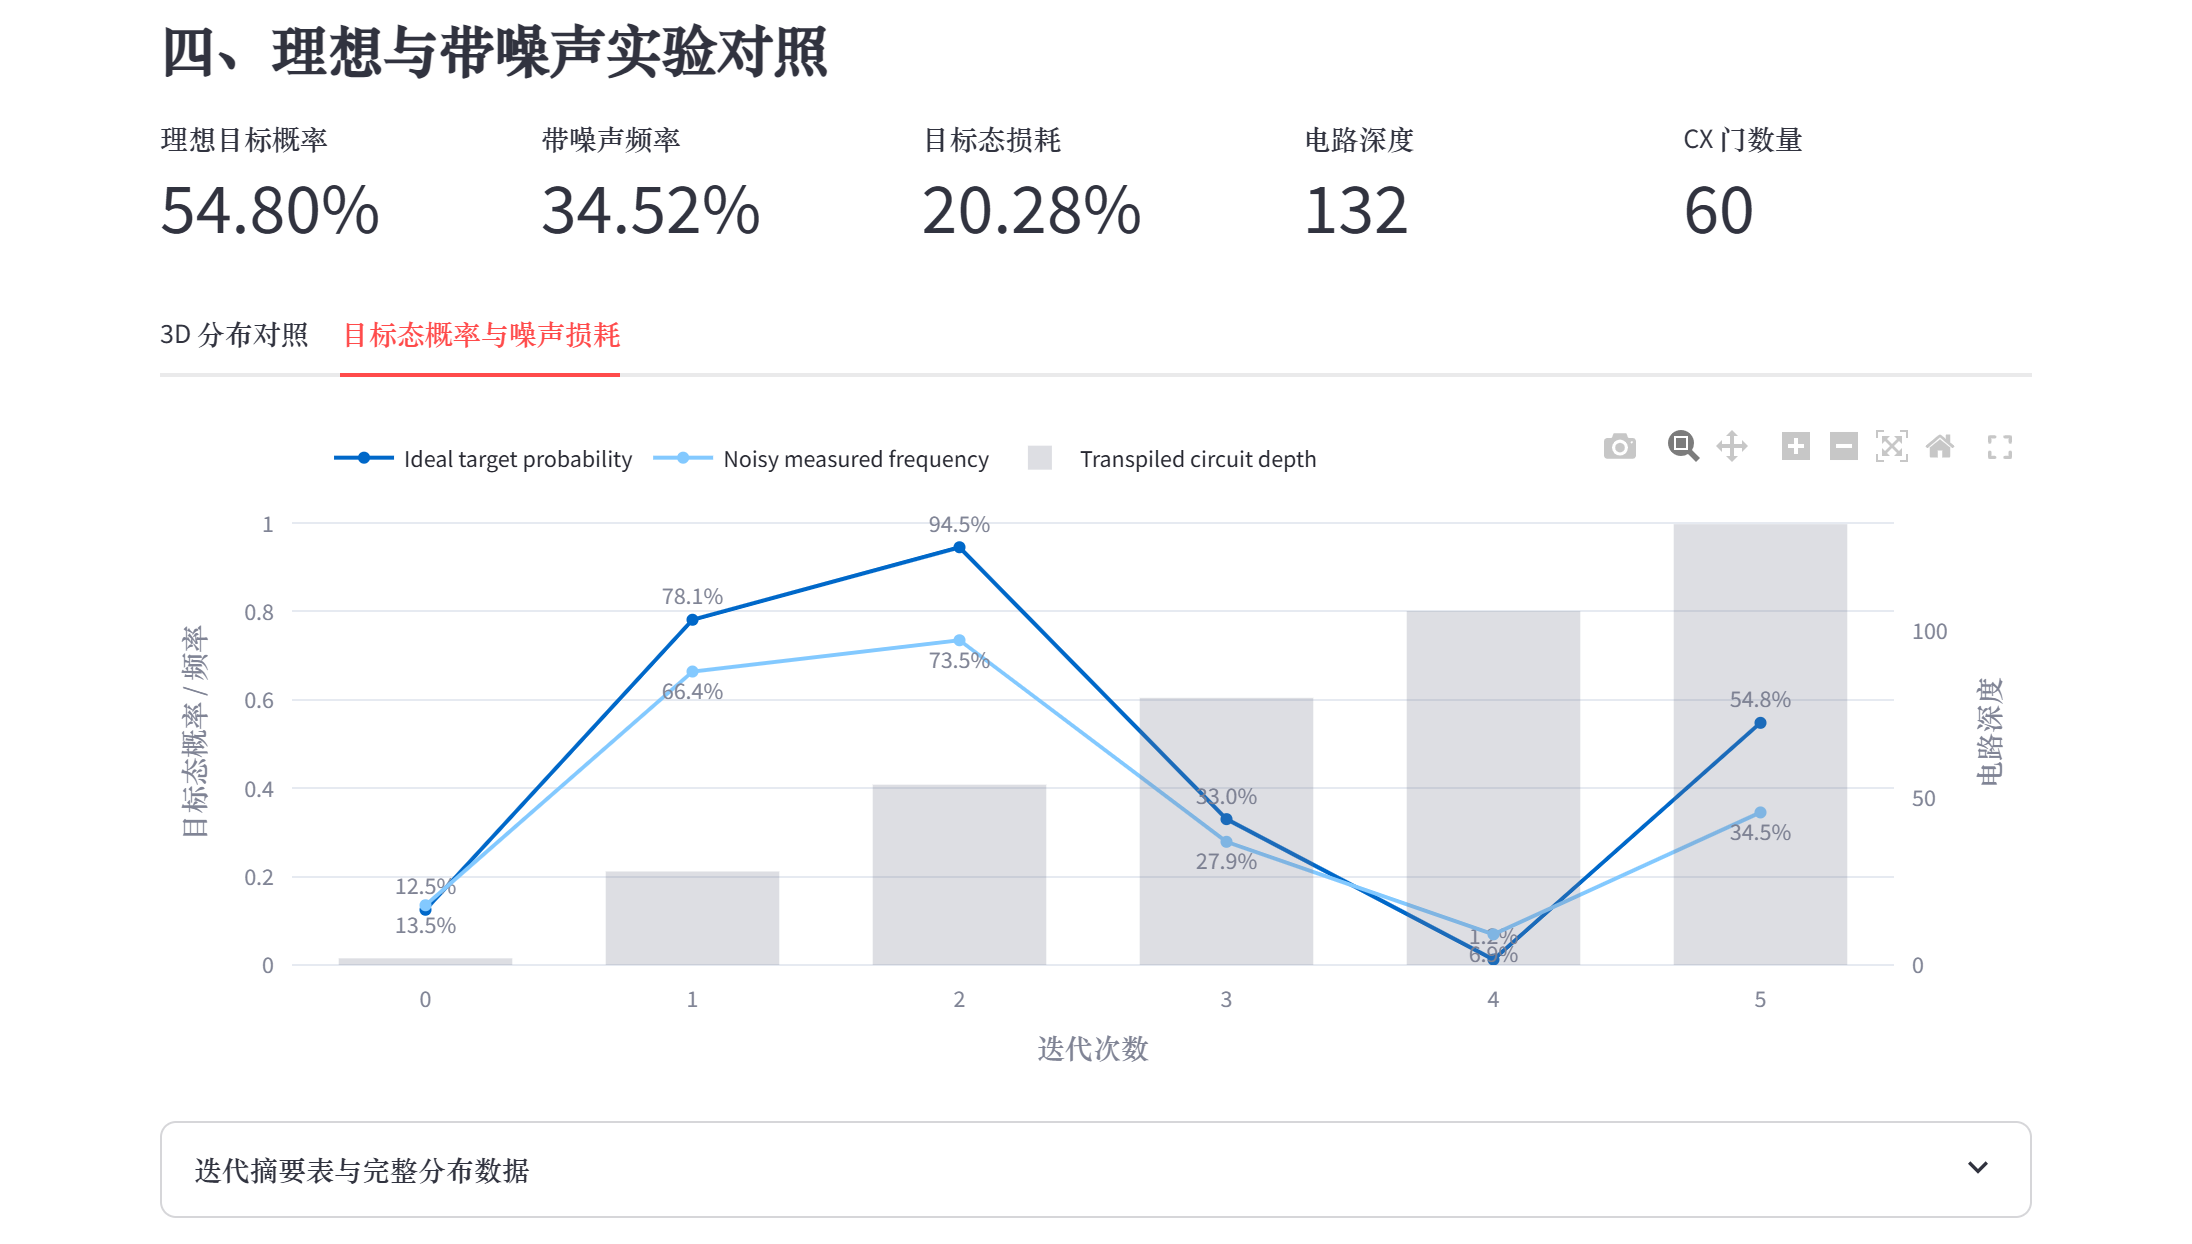
\includegraphics[width=0.95\textwidth]{images/web_crops/web_noise_view.png}
  }{
    \fbox{\parbox[c][5cm][c]{0.9\textwidth}{\centering 待插入理想与带噪声实验对照截图}}
  }
  \caption{理想概率分布与带噪声测量结果的对照视图}
  \label{fig:web-noise-view}
\end{figure}

\subsection{理论解释与错误迭代展示}

图~\ref{fig:web-theory-view}展示了页面中的理论解释区域。
该部分将Grover算法的理论概率公式、模拟结果和过迭代现象放在一起，
用于说明可视化结果与理论模型之间的对应关系。
对于单目标态搜索，目标态概率可以写为
\[
  P_r=\sin^2((2r+1)\theta),
\]
其中\(\sin(\theta)=1/\sqrt{N}\)。
页面根据当前量子比特数和目标态自动计算理论概率，并与程序模拟得到的目标态概率进行对照。

此外，页面还展示了错误迭代或过迭代时目标概率下降的现象，并说明Grover算法的振幅放大的周期性。

\begin{figure}[H]
  \centering
  \IfFileExists{images/web_crops/web_theory_view.png}{
    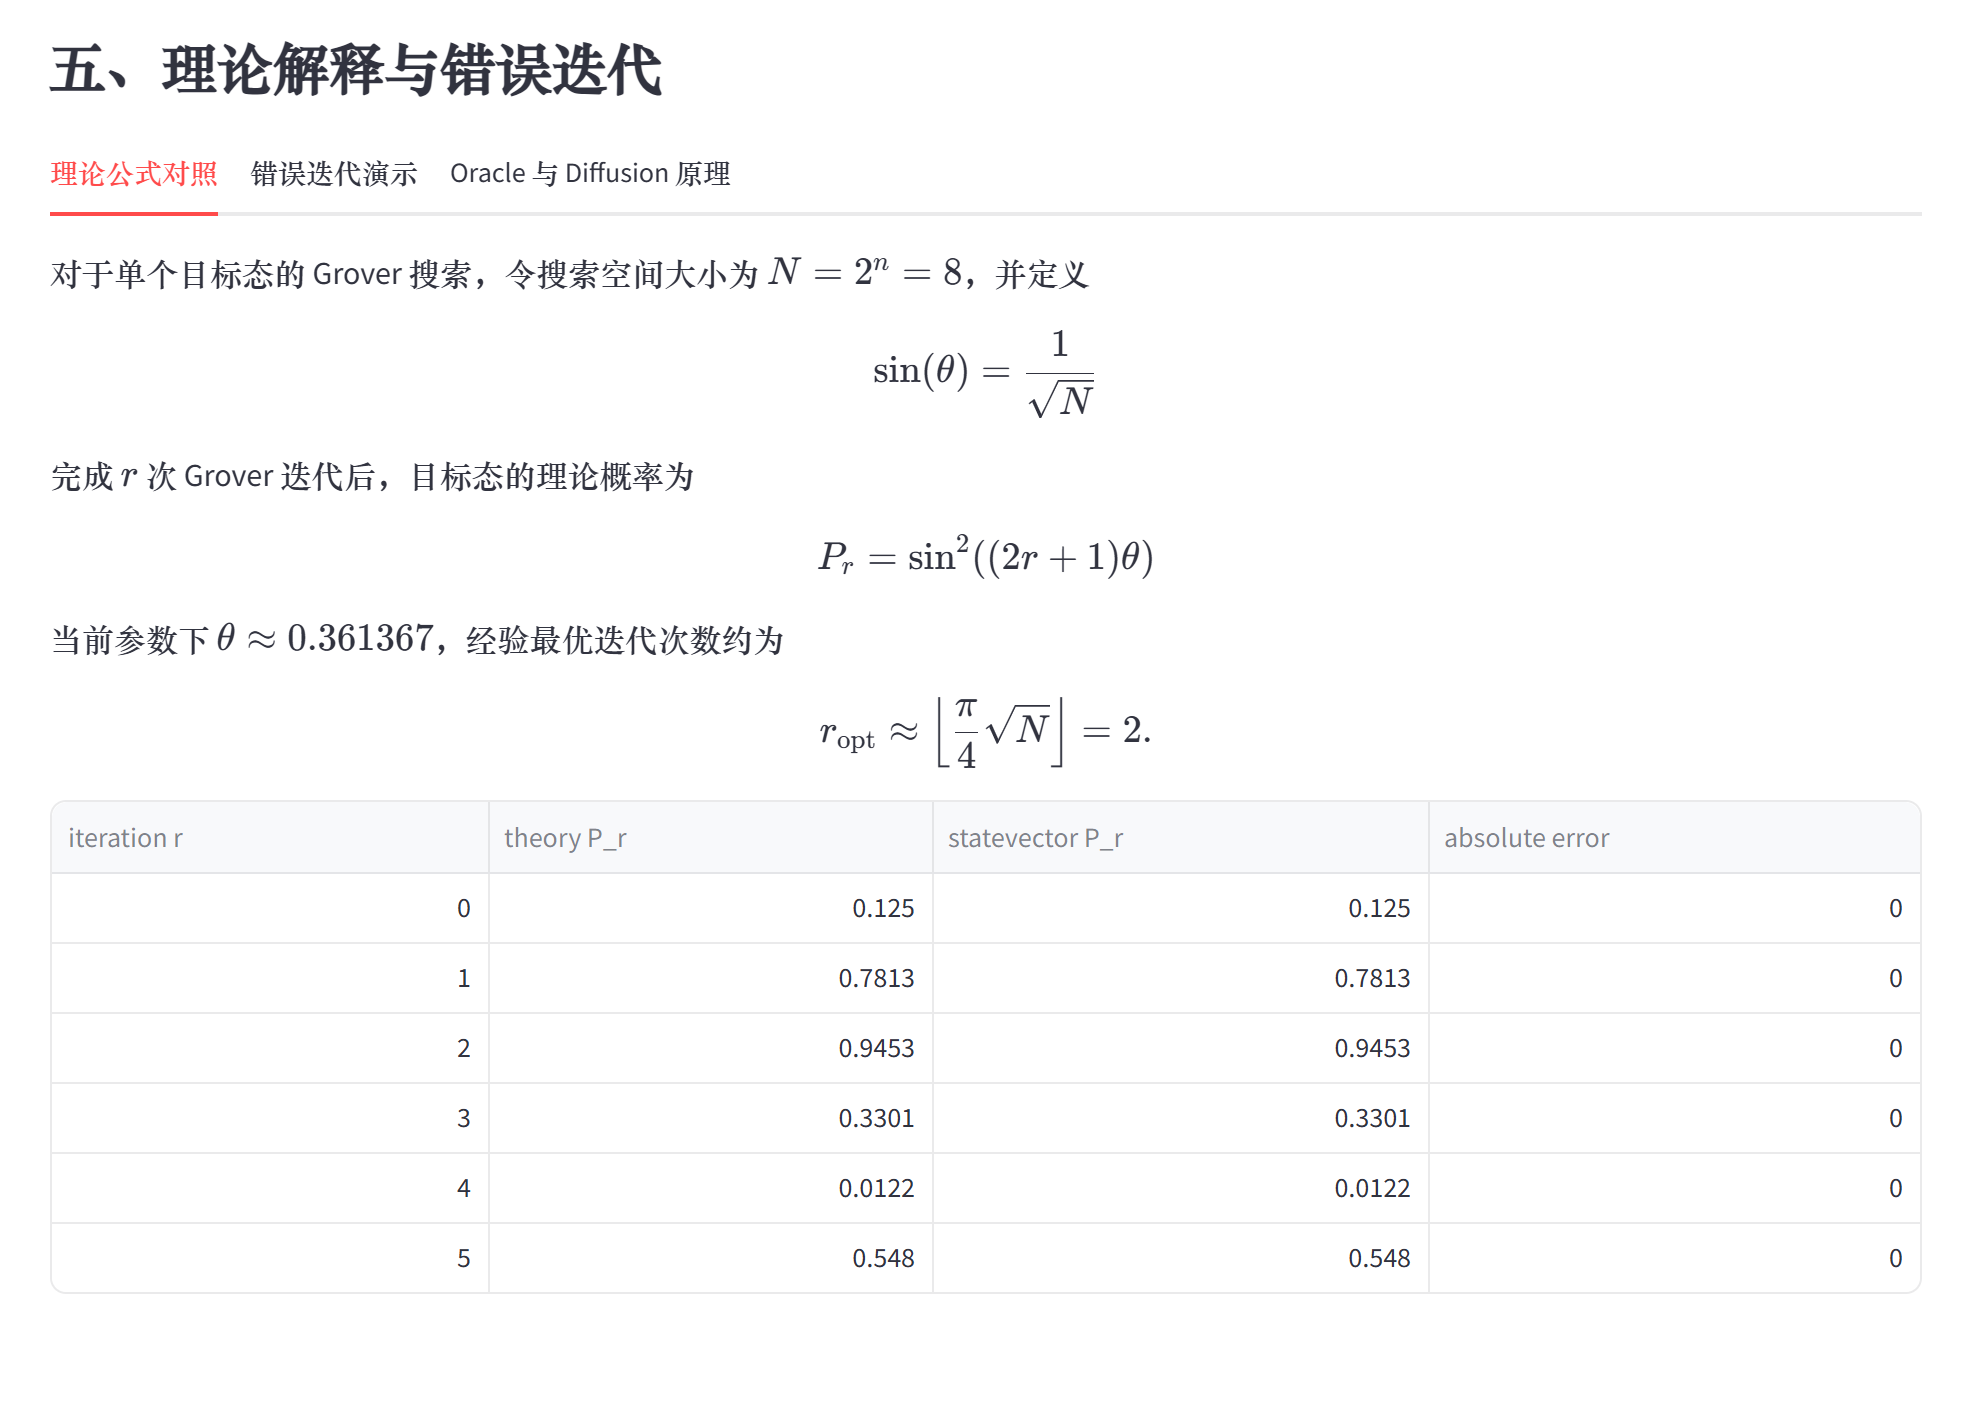
\includegraphics[width=0.95\textwidth]{images/web_crops/web_theory_view.png}
  }{
    \fbox{\parbox[c][5cm][c]{0.9\textwidth}{\centering 待插入理论解释与错误迭代截图}}
  }
  \caption{理论公式、模拟结果与过迭代现象的页面展示}
  \label{fig:web-theory-view}
\end{figure}
